\chapter{Creation of the Artifact}
\label{creation_of_the_artifact}

\section{Initial Goals}

As this project was first and foremost a project, designed to interactively explore the problemspace from the perspective of the \ac{HPC} community, 
all the while being contained by business requirements and time constraints, the initial goals of this project were very broad and open ended. 
At first the initial goal was simply to create a \ac{PoC} of a realistic workflow engine using the "Arkouda" project,
in order to present the Customer with a easily graspable example of its capabilities.

While we are approaching the problem from the perspective of the \ac{HPC} community, the intended enduser of this tool are the data scientists and \ac{SME}s 
that are working with the \ac{HPC} systems, and therefore the tool needs to be designed and selected with the fact in mind that the enduser will most likely not be knowledgeable in the field of \ac{HPC} or the underlying infrastructure.

In the first iteration of the project a preselection of possible Workflow management tools was given from the business side,
with the option to increase the scope if the presented tools were not sufficient.

Therefore the goals of the first iteration of this project was twofold, first to determine which, if any, of the presented tools were suitable for the task at hand,
and to determine what would make an adequate \ac{PoC} for the customer.

\section{Selection of Workflow Management Tools}

As described in the previous section, the first iteration of this project was to determine which, if any, of the presented tools were suitable for the task at hand.
The following section will describe the process of selecting the tools and the criteria that were used to evaluate them.
Because the time frame does not allow for a full integration and testing of all the presented tools in depth we will be using a decision making framework to evaluate the tools,
as described in the Methodologies \Ref{decision_making} to determine which tools will be most suitable for an initial \ac{PoC} and will serve as a good starting point for the project and future iterations.

\begin{itemize}
    \item \textbf{Pachyderm:} A \ac{k8s} based Workflow manager, written in go which was recently aquired by \ac{HPE}.
    \item \textbf{Argo:} A \ac{k8s} based Workflow manager , written in go, which is a \ac{CNCF} project \footcite{ArgoprojArgoworkflows2023}.
    \item \textbf{\ac{CLASP}:}  An in-house developed workflow manager, written in Java, utilizing Serverlet to execute workflows\footcite{sayersCloudApplicationServices2015}.
    \item \textbf{Snaplogic:} A commercial low-code/no-code workflow manager with a focus on data integration and data engineering\footcite{IPaaSSolutionEnterprise}.
\end{itemize}

But given that it was possible to select projects outside of the initial selection, the following projects also need to be considered:


\begin{itemize}
    \item \textbf{Airflow:} A Python-based workflow manager under the \ac{CNCF} umbrella, known for its easy-to-use interface and extensibility\footcite{hainesWorkflowOrchestrationApache2022}.
    \item \textbf{Kubeflow:} A \ac{k8s}-native platform for deploying, monitoring, and running ML workflows and experiments, also a \ac{CNCF} project, streamlining \ac{ML} operations alongside other Kubernetes resources \footcite{Kubeflow}.
    \item \textbf{Knative:} An open-source \ac{k8s}-based platform to build, deploy, and manage modern serverless workloads, simplifying the process of building cloud-native applications \footcite{HomeKnative}.
    \item \textbf{Luigi:} An open-source Python module created by Spotify to build complex pipelines of batch jobs, handling dependency resolution, workflow management, and visualization seamlessly \footcite{SpotifyLuigi2023}.
    \item \textbf{\ac{CWL}:} An open-standard for describing analysis workflows and tools in a way that makes them portable and scalable across a variety of software and hardware environments, from workstations to cluster, cloud, and high-performance computing environments.
\end{itemize}
    
% Why these tools??

\newpage
\subsubsection{Selection Criteria}

Due to this extensive list of diverse tools, a set of criteria was established to determine which tool would be the most suitable for the task at hand.
The following list of criteria was established to evaluate the tools:

\begin{itemize}
    \item \textbf{Ease of use:} 
        As the inted endusers of the tool are not primarily \ac{HPC} experts, the tool needs to be easy to use and understand,
        and should not require the enduser to have a deep understanding of the underlying infrastructure.
        While we can expect that the administration of the infrastructure will be done by adequately trained personnel, 
        the enduser should be spared having to adapt to the underlying infrastructure as much as possible.

    \item \textbf{Extensibility:}
        One significant constraint of the project is the restricted number of available work-hours.
        Given that the project's environment predominantly centers around HPC (High Performance Computing) workloads,
        it's essential for the tool to be easily expandable without requiring extensive modifications to the underlying system.
        Ideally this property would be transferred to the enduser, allowing them to easily extend the developed tool further to their needs.

    \item \textbf{Community, Support and  Documentation:}
        It is not enough that the software technically permits extensibility, the software also needs to be adequately documented and a support framework needs to be in place.
        Be it a community of users or a dedicated support team, the enduser and the developers need to be able to rely on the software being maintained and updated as well as being able to find expert help in case of problems.

    \item \textbf{Maturity:}
        With the boom of \ac{AI} and \ac{ML} in recent years \footcite{24TopAI}, the number of tools and frameworks has exploded, and while this is a good thing it also means that a lot of these tools are still paving their way and are developing rapidly.
        While this is not necessarily a bad thing, it does mean that the tool might not be ready for production use and might not be able to provide the stability and reliability that is required for a production environment or are lacking in documentation and support.      

    \item \textbf{Strategic alignment with \ac{HPE}:}
        As this project is being developed within the context of \ac{HPE}, it is important to consider the strategic alignment of the tool with \ac{HPE}.
        \ac{HPE} has is a large company with a diverse portfolio of products and services, and this project intersects with many different parts of the company.
        Therefore it is important to consider the strategic alignment of the tool with \ac{HPE} and its products and services.

    \item \textbf{License:}
        While this \ac{PoC} is not a commercial product in itself but rather an exploration of the problem space and a demonstration of what a final commercial product  might be like,
        it is important to consider the licenses of the tools that are being used.
        Having to strip out a tool later on because of licensing issues would be a significant setback and therefore needs to be considered.

    \item \textbf{Cost:}
        Time is not the only constraint of this project, as the project is being developed within the context of \ac{HPE} it is important to consider the cost of the tools that are being used.

\end{itemize}

\subsubsection{Weigting of the Criteria}

An integral part of the \ac{SMART} methodology is the weighting of the criteria, as described in section \ref{decision_making}.
In order to rank the criteria themselves, as they are quite hard to quantify, 
We will be using the weigting methodology as described in the \ac{SMART-ER} methodology \ref{acro:SMART-ER}.

The first step of which is the ranking of the criteria from most important to least important.

\begin{enumerate}
    \item \textbf{ Extensibility } As this is first and foremost a prototyping project, the actual development it at least for the first couple steps of the highest importance. 
    \item \textbf{ Community, Support \& Docs } This also applies for the external support available to the development team as if they are stuck, no developed can proceed, no matter the other factors.
    \item \textbf{ License } This criterion has to weighted carefully, as a highly restrictive license might be a dealbreaker, but a license that is too permissive might conflict with the strategic alignment with \ac{HPE}.
    \item \textbf{ Strategic alignment with \ac{HPE} } As this is developed by and for \ac{HPE} their requirements need to be consider aswell.
    \item \textbf{ Ease of Use } While the ease of use is important as this should eventually become a product, for now the central aspect is to create a \ac{PoC} therefore the usability is a priority, but not the highest.
    \item \textbf{ Cost } As this is a \ac{PoC} and not a commercial product, the cost is not the highest priority as this will be of small scale and therefore the cost will be negligible in most cases.
    \item \textbf{ Maturity } While the maturity of the tool is important, as this is a \ac{PoC} and not a commercial product, if the maturity of the tool does not impact the extensibility of the tool or the development process, it is not the highest priority.
\end{enumerate}



\begin{table}[htb]
    \centering
    \begin{tabular}{|l|l|} \hline
        \textbf{Criteria}                       & \textbf{Weight}       \\ \hline
        Extensibility                           & 0.3704                \\ \hline
        Community, Support and  Documentation   & 0.2276                \\ \hline
        License                                 & 0.1561                \\ \hline
        Strategic alignment with \ac{HPE}       & 0.1085                \\ \hline
        Ease of use                             & 0.0728                \\ \hline
        Maturity                                & 0.0442                \\ \hline
        Cost                                    & 0.0204                \\ \hline

    \end{tabular}
    \caption{Weighting of the criteria}
    \label{tab:weighting_of_the_criteria}
\end{table}


\subsubsection{Evaluation of the Tools}

The following table shows the evaluation of the tools which where suggested by the business, based on the criteria and the weighting of the criteria:

\begin{table}[htb]
    \centering
    \begin{tabular}{|l|l|l|l|l|} \hline
        \textbf{Criteria}                                          & \textbf{Pachyderm}    & \textbf{Argo}         & \textbf{\ac{CLASP}}   & \textbf{Snaplogic}     \\ \hline
        Ease of use                                                & TBD                   & TBD                   & TBD                   & TBD                    \\ \hline
        Extensibility                                              & TBD                   & TBD                   & TBD                   & TBD                    \\ \hline
        Community, Support \& Docs                                 & TBD                   & TBD                   & TBD                   & TBD                    \\ \hline
        Maturity                                                   & TBD                   & TBD                   & TBD                   & TBD                    \\ \hline
        Strategic alignment                                        & TBD                   & TBD                   & TBD                   & TBD                    \\ \hline
        License                                                    & TBD                   & TBD                   & TBD                   & TBD                    \\ \hline
        Cost                                                       & TBD                   & TBD                   & TBD                   & TBD                    \\ \hline

    \end{tabular}
    \caption{Evaluation of the suggested tools}
    \label{tab:evaluation_of_the_suggested_tools}
\end{table}

The following table shows the evaluation of the tools which where chosen for their relevance to the problem space, based on the criteria and the weighting of the criteria:

\begin{table}[htb]
    \centering
    \begin{tabular}{|l|l|l|l|l|l|} \hline
        \textbf{Criteria}                                          & \textbf{Airflow}      & \textbf{Kubeflow}     & \textbf{Knative}      & \textbf{Luigi}        & \textbf{CWL}          \\ \hline
        Ease of use                                                & TBD                   & TBD                   & TBD                   & TBD                   & TBD                   \\ \hline
        Extensibility                                              & TBD                   & TBD                   & TBD                   & TBD                   & TBD                   \\ \hline
        Community, Support \& Docs                                 & TBD                   & TBD                   & TBD                   & TBD                   & TBD                   \\ \hline
        Maturity                                                   & TBD                   & TBD                   & TBD                   & TBD                   & TBD                   \\ \hline
        Strategic alignment                                        & TBD                   & TBD                   & TBD                   & TBD                   & TBD                   \\ \hline
        License                                                    & TBD                   & TBD                   & TBD                   & TBD                   & TBD                   \\ \hline
        Cost                                                       & TBD                   & TBD                   & TBD                   & TBD                   & TBD                   \\ \hline

    \end{tabular}
    \caption{Evaluation of the additional tools}
    \label{tab:evaluation_of_the_additional_tools}
\end{table}




\section{Design of the Artifact}
 
As can be seen in figure \ref{abb:pachykouda_three_aspects}, the artifact is composed of 3 main components, 
the \textbf{Central Workflow Engine} which is responsible for the orchestration of the workflows (center),
the \textbf{\ac{HPC} Cluster} which is responsible for the execution of \ac{TCPP} workloads (left)
and the \textbf{Usability and Support Services} which aim at improving the usability and accessability for the enduser (right).

All this is build on top of the \textbf{Heydar Cluster} which has been specifically set up for this project and is described in more detail in section \ref{heydar_cluster}.


\begin{figure}[htb]
    \centering
    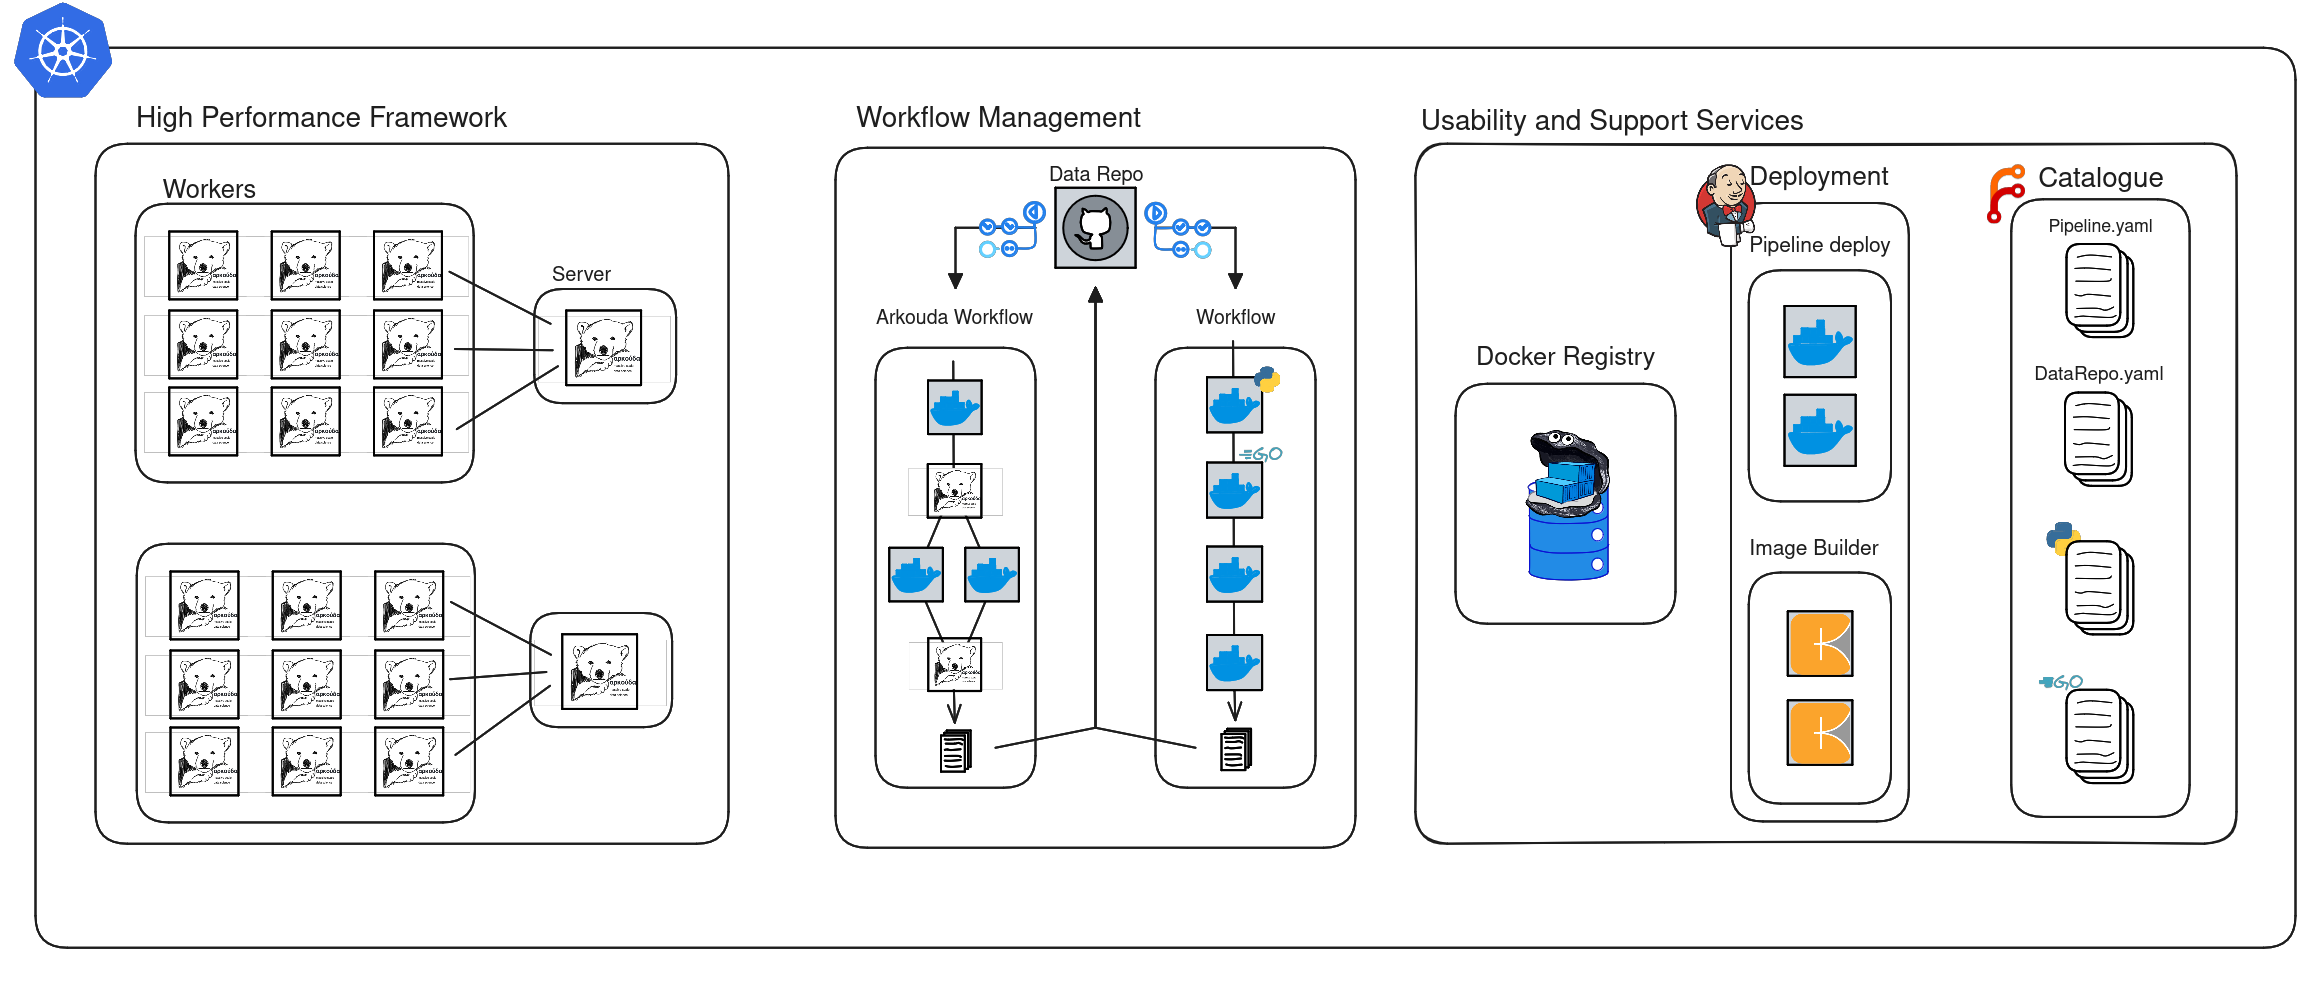
\includegraphics[width=16cm]{graphics/pachykouda_three_aspects.png}
    \caption[Pachykouda high level diagramm showing three main aspects]{Pachykouda high level infrastructure diagramm}
    \label{abb:pachykouda_three_aspects}
\end{figure}


\newpage


\section{Implementation of the Artifact}

This section will describe the iterative process of implementing the larger artifact and is broken up into 3 subsections.
While these steps where happening concurrently, they each address a different aspect of the project and therefore underwent their own iterative processes.


\subsection{Infrastructure}

\subsubsection{Minikube}

\subsubsection{Heydar Cluster}
\label{heydar_cluster}


\subsection{Usability Impovements}

\subsection{\ac{TCPP} Workloads } 


\newpage


\section{Evaluation of the Artifact}

\newpage
